\section{Federkonstante}

\subsection{Arbeitsgrundlagen}

Eine Stahlfeder kann mit der Formel
\begin{equation}
    F=F_0 + kz
    \label{eq:feder}
\end{equation}

beschrieben werden, wobei $k$ die Federkonstante ist, $z$ die Auslenkung in meter ist, $F_0$ die
Vorspannung ist, und $F$ die ben\"otigte Kraft ist.


\subsection{Durchf\"uhrung}

\subsubsection*{Versuchsanordnung}

Die Kraft und die Distanz einer Stahlfeder wurde bei verschiedenen Auslenkungen gemessen.


\subsubsection*{Messergebnisse}

\begin{center}
    \begin{threeparttable}
        \caption{Gemessene Gr\"ossen}
        \begin{tabular}{ccc}
            \toprule
            $F (N)$ & \hspace{12mm} & $z (m)$ \\
            \midrule
            4.14  & & 0.20 \\
            6.36  & & 0.35 \\
            7.92  & & 0.42 \\
            9.86  & & 0.46 \\
            11.11 & & 0.51 \\
            11.70 & & 0.54 \\
            12.76 & & 0.59 \\
            14.21 & & 0.67 \\
            15.29 & & 0.71 \\
            16.98 & & 0.80 \\
            \bottomrule
        \end{tabular}
        \begin{tablenotes}
            \small
            \item \textbf{Hinweis:} Daten wurden vom Auftragsdokument kopiert.
        \end{tablenotes}
        \label{tab:feder}
    \end{threeparttable}
\end{center}

Die Federkonstante $k$ und die Vorspannkraft $F_0$ soll durch lineare Regression ermittelt werden.


\subsubsection*{Berechnung mit dem Taschenrechner}

Es werden zwei unbekannte Gr\"ossen $k$ und $F_0$ in der linearen Funktion $\bar{F}=\bar{z}k+F_0$
f\"ur die Messpaare $(F_i, z_i)$ gesucht. $k$ l\"asst sich mit der Formel
\begin{equation}
    k = \frac{ \sum_{i=1}^{N} (z_i - \bar{z}) (F_i - \bar{F})}{ \sum_{i=1}^{N} (z_i - \bar{z})^2} = \SI{22.53}{\newton\per\meter}
    \label{eq:k}
\end{equation}

berechnen, wobei $F_i$ und $z_i$ die Messpaare von der Tabelle \ref{tab:feder} sind, $N=10$, und
$\bar{F}$ und $\bar{z}$ die Mittelwerte aller Werte $F_i$ und $z_i$ sind. Die Mittelwerte von
$F_i$ und $z_i$ k\"onnen mit der Formel
der Formel
\begin{equation}
    \bar{x} = \frac{1}{N} \sum_{i=1}^{N} x_i
    \label{eq:mittelwert}
\end{equation}
berechnet werden.

Durch Umformen der linearen Funktion in der Formel \ref{eq:feder} kann nun auch $F_0$ berechnet
werden.
\begin{equation}
    F_0 = \bar{F} - k\bar{z} = \SI{-0.79}{\newton}
\end{equation}


\subsubsection*{QtiPlot}

\begin{figure}[H]
    \center
    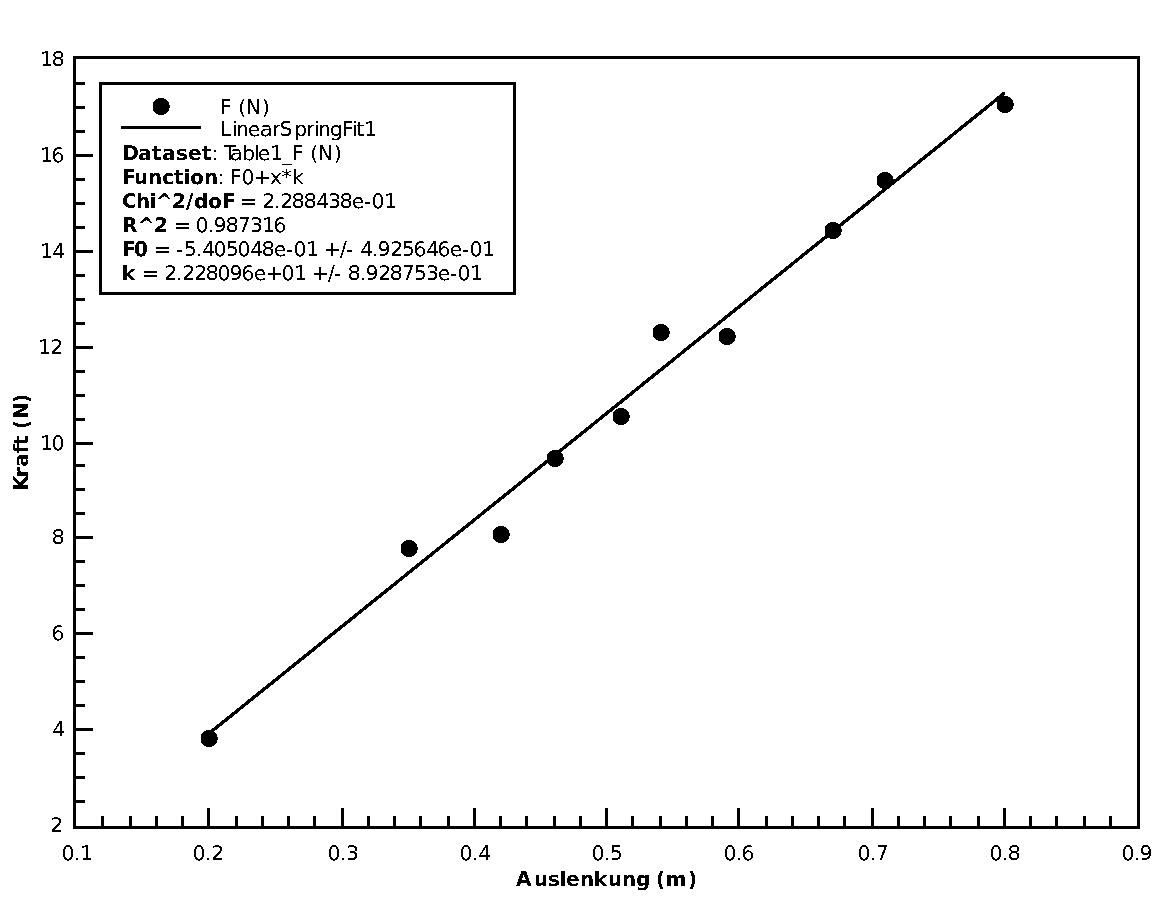
\includegraphics[width=.8\textwidth]{qtiplot/feder-linear}
    \caption{Lineare Regression zur Bestimmung von $k$ und $F_0$}
    \label{fig:feder-linear}
\end{figure}

\begin{figure}[H]
    \center
    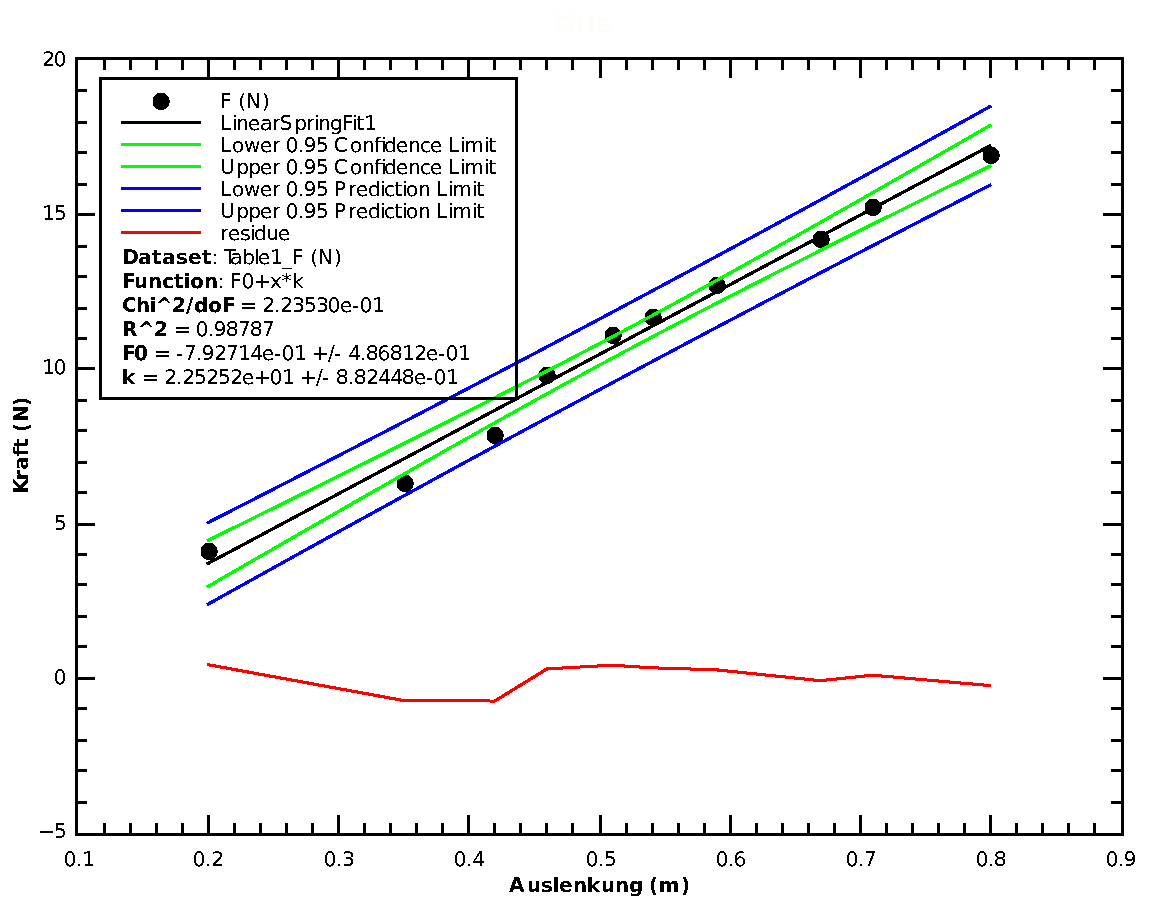
\includegraphics[width=.8\textwidth]{qtiplot/feder-95-bands}
    \caption{95\% Confidence- und Prediction-bands sowie Residuals}
    \label{fig:feder-95-bands}
\end{figure}

\begin{figure}[H]
    \center
    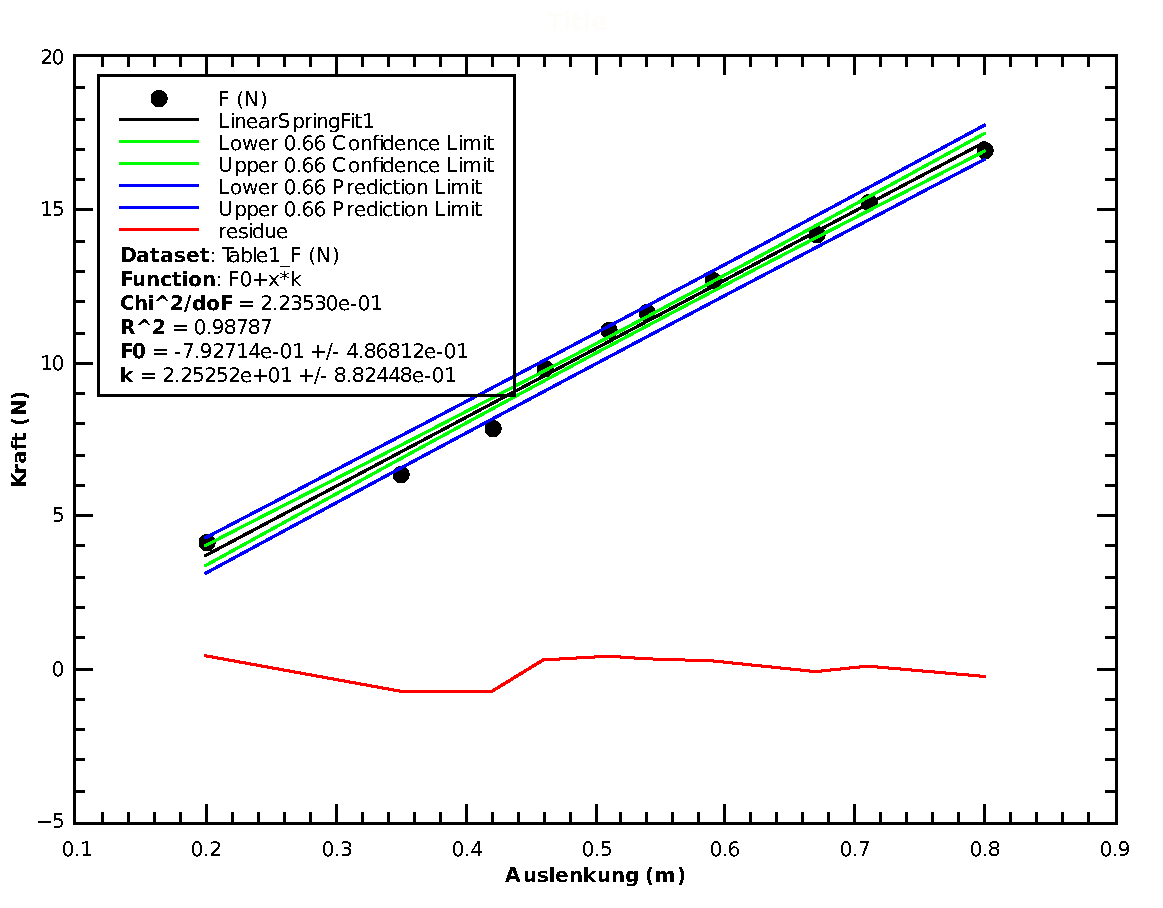
\includegraphics[width=.8\textwidth]{qtiplot/feder-66-bands}
    \caption{66\% Confidence- und Prediction-bands sowie Residuals}
    \label{fig:feder-66-bands}
\end{figure}


\subsection{Resultate und Diskussion}

Die mit dem Taschenrechner erhaltenen Werte stimmen mit den Werten von QtiPlot \"uberein.

Ein Fehler, den ich zuerst gemacht habe, war es, die X und Y Achsen in QtiPlot zu vertauschen,
sprich, $F_i$ auf die X-Achse und $z_i$ auf die Y-Achse. Dadurch sind zuerst die falschen Werte
von $k$ und $F_0$ berechnet worden.

